\section{Preliminaries}\label{sect:prelim}

In this section, we review the basics of matrix Schubert varieties as well as the CDG generators introduced in \cite{HPW}.  For a more detailed introduction to matrix Schubert varieties, we refer the reader to \cite[Chapter 10]{Ful96}.  For basic properties of and standard terminology for Gr\"obner bases, we refer the reader to \cite{Eis95}.  

\subsection{Matrix Schubert varieties}\label{subsect:MSv}

We begin by describing how each permutation is associated to the affine variety called a matrix Schubert variety.  Throughout this paper, we will take  $[n] = \{1,2,\dots,n\}$  for any $n \geq 1$ and let $S_n$ denote the symmetric group on $[n]$.  Each permutation $w \in S_n$ is a bijection $w:[n] \rightarrow [n]$, which we will record in its one-line notation $w = w_1 w_2 \dots w_n$ where $w_i = w(i)$.  To every $w \in S_n$, we associate a \emph{Rothe diagram} $D_w$, defined as follows:
\[
D_w = \{(i,j) \in [n] \times [n]: w(i) > j, w^{-1}(j) > i\}.
\]
A Rothe diagram has the following visualization: In an $n \times n$ grid, place a $\bullet$ in position $(i,w_i)$ for each $i \in [n]$, and draw a line down from each $\bullet$ to the bottom of the grid and a line to the right from each $\bullet$ to the side of the grid.  Then $D_w$ is the set of boxes in the grid without a $\bullet$ in them or a line through them.
For example, $D_{315642}$ is the set $\{(1,1),(1,2),(3,2),(3,4),(4,2),(4,4),(5,2)\}$ and corresponds to the visualization below, in which the elements of $D_{315642}$ appear in gray and will be referred to as the \emph{boxes} of $w$:
\[
  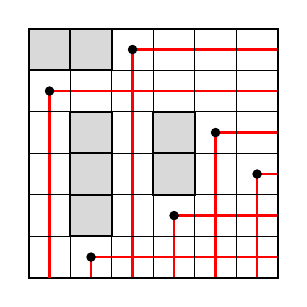
\begin{tikzpicture}[x=1.5em,y=1.5em]
      \draw[color=black, thick](0,1)rectangle(6,7);
     \filldraw[color=black, fill=gray!30, thick](0,6)rectangle(1,7);
      \filldraw[color=black, fill=gray!30, thick](1,6)rectangle(2,7);
      \filldraw[color=black, fill=gray!30, thick](1,4)rectangle(2,5);
      \filldraw[color=black, fill=gray!30, thick](3,4)rectangle(4,5);
       \filldraw[color=black, fill=gray!30, thick](1,3)rectangle(2,4);
      \filldraw[color=black, fill=gray!30, thick](3,3)rectangle(4,4);
      \filldraw[color=black, fill=gray!30, thick](1,2)rectangle(2,3);      
     \draw[thick,color=red] (6,6.5)--(2.5,6.5)--(2.5,1);
     \draw[thick,color=red] (6,5.5)--(0.5,5.5)--(0.5,1);
     \draw[thick,color=red] (6,4.5)--(4.5,4.5)--(4.5,1);
     \draw[thick,color=red] (6,3.5)--(5.5,3.5)--(5.5,1);
     \draw[thick,color=red] (6,2.5)--(3.5,2.5)--(3.5,1);
     \draw[thick,color=red] (6,1.5)--(1.5,1.5)--(1.5,1);
     \filldraw [black](2.5,6.5)circle(.1);
     \filldraw [black](0.5,5.5)circle(.1);
      \filldraw [black](4.5,4.5)circle(.1);
     \filldraw [black](5.5,3.5)circle(.1);
     \filldraw [black](3.5,2.5)circle(.1);
      \filldraw [black](1.5,1.5)circle(.1);
      \draw[color=black](2,6)rectangle(3,7);
      \draw[color=black](3,6)rectangle(4,7); 
      \draw[color=black](4,6)rectangle(5,7);
      \draw[color=black](5,6)rectangle(6,7); 
      \draw[color=black](0,5)rectangle(1,6);
      \draw[color=black](1,5)rectangle(2,6);  
      \draw[color=black](2,5)rectangle(3,6);
      \draw[color=black](3,5)rectangle(4,6); 
      \draw[color=black](4,5)rectangle(5,6);
      \draw[color=black](5,5)rectangle(6,6); 
     \draw[color=black](0,4)rectangle(1,5); 
      \draw[color=black](2,4)rectangle(3,5);
      \draw[color=black](4,4)rectangle(5,5);
      \draw[color=black](5,4)rectangle(6,5); 
      \draw[color=black](0,3)rectangle(1,4); 
      \draw[color=black](2,3)rectangle(3,4);
      \draw[color=black](4,3)rectangle(5,4);
      \draw[color=black](5,3)rectangle(6,4); 
      \draw[color=black](0,2)rectangle(1,3); 
      \draw[color=black](2,2)rectangle(3,3);
      \draw[color=black](3,2)rectangle(4,3);
      \draw[color=black](4,2)rectangle(5,3);
      \draw[color=black](5,2)rectangle(6,3); 
      \draw[color=black](1,1)rectangle(2,2);  
      \draw[color=black](2,1)rectangle(3,2);
      \draw[color=black](3,1)rectangle(4,2); 
      \draw[color=black](4,1)rectangle(5,2);
      \draw[color=black](5,1)rectangle(6,2); 
     \end{tikzpicture}.
\]

The \emph{Coxeter length} of the permutation $w$ is equal to its inversion number, i.e. 
\[| \{ (i, j) \mid i < j, w_i > w_j \}|,
\] which is in turn equal to $|D_w|$.  For example, the Coxeter length of $315642$ is $7$, easily read off as the number of gray boxes in the diagram above.

\begin{definition}
Fix a permutation $w = w_1 \cdots w_n \in S_n$ and a permutation $v  = v_1\ldots v_k \in S_k$ with $k \leq n$.  If there is some substring $w_{i_1} \cdots w_{i_k}$ of $w$ satisfying $w_{i_j} < w_{i_\ell}$ exactly when $v_j < v_\ell$, then we say that $w$ \emph{contains} $v$.  Otherwise, we say that $w$ \emph{avoids} $v$.
\end{definition}

For example, $w = 13254$ contains $v = 2143$ with $3254$ the substring of $w$ realizing the containment, but $w$ does not contain $v' = 3214$.  Notice that if $w_{i_1} \cdots w_{i_k}$ satisfies $w_{i_j} < w_{i_\ell}$ exactly when $v_j < v_\ell$, then the Rothe diagram of $v$ can be obtained from that of $w$ by restricting to the rows $i_1, \ldots, i_k$ and columns $w_{i_1}, \ldots, w_{i_k}$ in the $[n] \times [n]$ grid giving the visualization of $D_w$.  

By restricting to the maximally southeast boxes of connected components of $D_w$, we define the \emph{essential set} of $w$: 
\[
\Ess(w) = \{(i,j) \in D_w \mid (i+1,j), (i,j+1) \notin D_w\}.
\]
In the example above, $\Ess(315642)=\{(1,2),(4,4), (5,2)\}$.  Borrowing a term from the literature on ladder determinantal varieties, if $(i,j) \in \Ess(w)$ and there is no $(i'j') \in \Ess(w)$ with $i \leq i'$, $j \leq j'$, and $(i,j) \neq (i',j')$, we will say that $(i,j)$ is a \emph{lower outside corner} of $D_w$.  In the case of $w = 315642$, $(4,4)$ and $(5,2)$ are lower outside corners, but $(1,2)$ is not.  

To every permutation $w \in S_n$, we associate a \emph{rank function} $\rank_w : [n] \times [n] \to \mathbb{Z}$, where 
\[
\rank_w(i,j) = |\{k \leq i \mid w(k) \leq j\}|,
\] and the rank matrix $M_w$ whose $(i,j)^{th}$ entry is $\rank_w(i,j)$.  Visually, we assign to every square $(i,j)$ in the $[n] \times [n]$ grid underlying the Rothe diagram of $w$ the number of $\bullet$s weakly northwest of $(i,j)$.  In our running example $w = 315642$, one may find it helpful to record the information as  \definecolor{burntorange}{rgb}{0.8, 0.33, 0.0}
\[
\begin{minipage}{0.4\textwidth}\
\[
\hspace{1cm} M_w = \begin{bmatrix}
\boxed{0} & {\color{burntorange}\boxed{0}} & 1 & 1 & 1 & 1\\
1 & 1 & 2 & 2 & 2 & 2\\
1 & \boxed{1} & 2 & \boxed{2} & 3 & 3\\
1 & \boxed{1} & 2 & {\color{burntorange}\boxed{2}} & 3 & 4\\
1 & {\color{burntorange}\boxed{1}} & 2 & 3 & 4 & 5\\
1 & 2 & 3 & 4 & 5 & 6\\
\end{bmatrix} 
\]

\end{minipage} \hspace{1cm} \mbox{ or as } \hspace{0.6cm} \begin{minipage}{.4\textwidth}
\hspace{0.5cm} 
  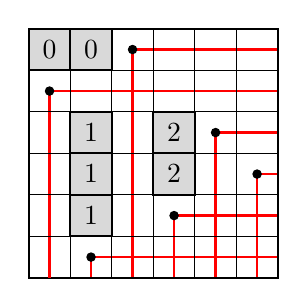
\begin{tikzpicture}[x=1.5em,y=1.5em]
      \draw[color=black, thick](0,1)rectangle(6,7);
     \filldraw[color=black, fill=gray!30, thick](0,6)rectangle(1,7);
      \filldraw[color=black, fill=gray!30, thick](1,6)rectangle(2,7);
      \filldraw[color=black, fill=gray!30, thick](1,4)rectangle(2,5);
      \filldraw[color=black, fill=gray!30, thick](3,4)rectangle(4,5);
       \filldraw[color=black, fill=gray!30, thick](1,3)rectangle(2,4);
      \filldraw[color=black, fill=gray!30, thick](3,3)rectangle(4,4);
      \filldraw[color=black, fill=gray!30, thick](1,2)rectangle(2,3);      
     \draw[thick,color=red] (6,6.5)--(2.5,6.5)--(2.5,1);
     \draw[thick,color=red] (6,5.5)--(0.5,5.5)--(0.5,1);
     \draw[thick,color=red] (6,4.5)--(4.5,4.5)--(4.5,1);
     \draw[thick,color=red] (6,3.5)--(5.5,3.5)--(5.5,1);
     \draw[thick,color=red] (6,2.5)--(3.5,2.5)--(3.5,1);
     \draw[thick,color=red] (6,1.5)--(1.5,1.5)--(1.5,1);
     \filldraw [black](2.5,6.5)circle(.1);
     \filldraw [black](0.5,5.5)circle(.1);
      \filldraw [black](4.5,4.5)circle(.1);
     \filldraw [black](5.5,3.5)circle(.1);
     \filldraw [black](3.5,2.5)circle(.1);
      \filldraw [black](1.5,1.5)circle(.1);
      \draw[color=black](2,6)rectangle(3,7);
      \draw[color=black](3,6)rectangle(4,7); 
      \draw[color=black](4,6)rectangle(5,7);
      \draw[color=black](5,6)rectangle(6,7); 
      \draw[color=black](0,5)rectangle(1,6);
      \draw[color=black](1,5)rectangle(2,6);  
      \draw[color=black](2,5)rectangle(3,6);
      \draw[color=black](3,5)rectangle(4,6); 
      \draw[color=black](4,5)rectangle(5,6);
      \draw[color=black](5,5)rectangle(6,6); 
     \draw[color=black](0,4)rectangle(1,5); 
      \draw[color=black](2,4)rectangle(3,5);
      \draw[color=black](4,4)rectangle(5,5);
      \draw[color=black](5,4)rectangle(6,5); 
      \draw[color=black](0,3)rectangle(1,4); 
      \draw[color=black](2,3)rectangle(3,4);
      \draw[color=black](4,3)rectangle(5,4);
      \draw[color=black](5,3)rectangle(6,4); 
      \draw[color=black](0,2)rectangle(1,3); 
      \draw[color=black](2,2)rectangle(3,3);
      \draw[color=black](3,2)rectangle(4,3);
      \draw[color=black](4,2)rectangle(5,3);
      \draw[color=black](5,2)rectangle(6,3); 
      \draw[color=black](1,1)rectangle(2,2);  
      \draw[color=black](2,1)rectangle(3,2);
      \draw[color=black](3,1)rectangle(4,2); 
      \draw[color=black](4,1)rectangle(5,2);
      \draw[color=black](5,1)rectangle(6,2); 
     \node at (0.5,6.5) {$0$};
      \node at (1.5,6.5) {$0$};
      \node at (1.5,4.5) {$1$};
      \node at (1.5,3.5) {$1$};
      \node at (1.5,2.5) {$1$};
       \node at (3.5,4.5) {$2$};
       \node at (3.5,3.5) {$2$};
     \end{tikzpicture}.
  \end{minipage}   
       \]
Note that the transpose of the rank matrix of $w$ and transpose of the Rothe diagram of $w$ correspond to the rank matrix and Rothe diagram of $w^{-1}$, respectively, because the inverse of a permutation matrix is its transpose.  We have recorded elements of $D_w$ in the rank matrix $M_w$ as boxes and colored the boxes of the essential set orange in anticipation of our discussion of Fulton generators, below.

Let $\mbox{Mat}_{n,n}$ denote the affine $n^2$-space of complex $n \times n$ matrices.  Given $N \in \mbox{Mat}_{n,n}$ and subsets $A,B \subseteq [n]$, let $N_{A,B}$ be the submatrix of $N$ determined by the rows whose indices are elements of $A$ and the columns whose indices are elements of $B$.  Then the \emph{matrix Schubert variety} of $w \in S_n$ is the affine variety \[
X_w = \left\{Z \in \mbox{Mat}_{n,n}\mid \rank{Z_{[i],[j]}} \leq \rank_w(i,j)\ \mbox{for all}\ (i,j) \in [n] \times [n] \right\}.
\]

Let $Z = (z_{i,j})_{(i,j) \in [n] \times [n]}$ be a matrix of distinct indeterminates and $R = \mathbb{C}[Z]$ so that $\Spec(R)$ is identified with $\mbox{Mat}_{n,n}$.  The \emph{Schubert determinantal ideal} of $w$ is 
\[
I_w = ( (\rank_w(i,j)+1)\text{-minors in } Z_{[i],[j]} \mid (i,j) \in [n] \times [n] ) \subseteq R.
\]  This naive generating set will typically include a good deal of redundancy, and so we will more often consider the smaller set of \emph{Fulton generators} of $I_w$: \[
	\{(\rank_w(i,j)+1)\text{-minors in } Z_{[i],[j]} \mid (i,j) \in \Ess(w) \}.
\]  Fulton showed that the Fulton generators indeed generate $I_w$ \cite[Lemma 3.10]{Ful92}, that $I_w$ is prime, and, in particular, that $X_w \cong \Spec(R/I_w)$ as reduced schemes  \cite[Proposition 3.3]{Ful92}.  The height of the ideal $I_w$ (equivalently, codimension of $\Spec(R/I_w)$ in $\Spec(R)$) is equal to the Coxeter length of $w$ \cite[Proposition 3.3]{Ful92}.

In the example $w = 315642$, the Fulton generators of $I_w$ are $z_{1,1}$, $z_{1,2}$, the $2$-minors of \begin{center} $\begin{bmatrix}
z_{1,1} & z_{1,2}\\
z_{2,1} & z_{2,2}\\
z_{3,1} & z_{3,2}\\
z_{4,1} & z_{4,2}\\
z_{5,1} & z_{5,2}\\
\end{bmatrix},
$ and the $3$-minors of  $\begin{bmatrix}
z_{1,1} & z_{1,2} & z_{1,3} & z_{1,4}\\
z_{2,1} & z_{2,2} & z_{2,3} & z_{2,4}\\
z_{3,1} & z_{3,2} & z_{3,3} & z_{3,4}\\
z_{4,1} & z_{4,2} & z_{4,3} & z_{4,4}\\
\end{bmatrix}.
$ \end{center} 

\subsection{CDG generators}\label{subsect:CDG}

In \cite{HPW}, the authors introduce \emph{CDG generators} of defining ideals of matrix Schubert varieties.  These generators are named after Conca, De Negri, and Gorla, whose result \cite[Theorem 4.2]{CDG15} served as inspiration for the generating set used in \cite{HPW} and, in particular, for Conjecture \ref{conj:mainresult}.

\begin{definition}
Fix a permutation $w \in S_n$ and an $n \times n$ matrix $Z = (z_{i,j})_{(i,j) \in [n] \times [n]}$ of distinct indeterminates.  Let $\Dom(w) = \{(i,j) \in D_w \mid \rank_w(i,j) = 0\}$, and call $\Dom(w)$ the \emph{dominant part} of the Rothe diagram $D_w$.  From $Z$, form the matrix $Z'$ by replacing $z_{i,j}$ by $0$ whenever $(i,j) \in \Dom(w)$.  Set \[
	G'_w = \{(\rank_w(i,j)+1)\text{-minors in } Z'_{[i],[j]} \mid (i,j) \in \Ess(w)\setminus \Dom(w) \},
\] and $G_w = G'_w \cup \{z_{i,j} \mid (i,j) \in \Dom(w)\}$.  We call $G_w$ the set of \emph{CDG generators} of $I_w$.
\end{definition}

\begin{example}
If $w = 315642$ the CDG generators of $I_w$ are $z_{1,1}$, $z_{1,2}$, the $2$-minors of \begin{center} $\begin{bmatrix}
0 & 0\\
z_{2,1} & z_{2,2}\\
z_{3,1} & z_{3,2}\\
z_{4,1} & z_{4,2}\\
z_{5,1} & z_{5,2}\\
\end{bmatrix},
$ and the $3$-minors of  $\begin{bmatrix}
0 & 0 & z_{1,3} & z_{1,4}\\
z_{2,1} & z_{2,2} & z_{2,3} & z_{2,4}\\
z_{3,1} & z_{3,2} & z_{3,3} & z_{3,4}\\
z_{4,1} & z_{4,2} & z_{4,3} & z_{4,4}\\
\end{bmatrix}.
$ \end{center}
\end{example}

\noindent Notice that $\Dom(w) = \emptyset$ if and only if $w_1 = 1$, in which case the CDG generators and the Fulton generators coincide.  

\subsection{Gr\"obner bases}\label{subsect:Grobner}

Let $S=\mathbb{C}[x_1, \ldots, x_d]$.  A \emph{term order} $<$ on $S$ is a total order on the monic monomials of $S$ so that $1 \leq \mu$ for every monomial $\mu$ of $S$ and so that, for all monomials $\mu_1, \mu_2$, and $\nu$, $\mu_1<\mu_2$ implies $\mu_1 \nu < \mu_2 \nu$.  Let $f = \sum_{i=1}^k c_i \mu_i \in S$ where $c_i \in \CC$ and the $\mu_i$ are monic monomials (written in the usual way so that $\mu_i \neq \mu_j$ whenever $i \neq j$ and no $c_i$ is  $0$).  Fix $i$ so that $c_i \mu_i >c_j \mu_j$ whenever $i \neq j$, and define the \emph{leading term} of $f$ to be $LT(f)=c_i \mu_i$.  For an ideal $I$ of $S$, define the \emph{initial ideal} of $I$ to be $LT(I) = (LT(f) \mid f \in I)$.  A generating set $\mathcal{G}$ of $I$ is called a \emph{Gr\"obner basis} if $LT(I) = (LT(g) \mid g \in \mathcal{G})$.  For a detailed introduction to the theory of Gr\"obner bases, including Buchberger's algorithm, we refer the reader to \cite[Chapter 15]{Eis95}.

\begin{definition}
When the set of CDG generators forms a Gr\"obner basis for the Schubert determinantal ideal $I_w$ under every diagonal term order, we will say that the permutation \emph{$w$ is CDG}.  
\end{definition}

\section{Rothe diagrams of CDG permutations}\label{sect:backward}

\subsection{Obstructions to being CDG}

We begin this section by describing in terms of the Rothe diagram $D_w$ conditions that prevent $w$ from being CDG.  In Subsection \ref{subsect:backward}, we will show that when $D_w$ does not satisfy these conditions, $w$ is necessarily CDG.

Before we begin, we note that the visualization of the Rothe diagram of $214635$ is obtained from that of $215364$ by transposition.  The same is true of $315264$ and $241635$.  The visualizations of the Rothe diagrams of the remaining permutations listed in Conjecture \ref{conj:mainresult} are self transpose.   This symmetry will allow us to consolidate some of our case work below.  We understand the cardinal directions in reference to $D_w$ in terms of its visualization.  We say, for example, that $(i',j')$ is ``strictly southeast" of $(i,j)$ to mean that both $i'>i$ and also $j'>j$, or that $(i',j')$ is ``strictly south and weakly east" of $(i,j)$ to mean $i'>i$ and also $j' \geq j$.

\begin{definition}
The permutation $w$ has an \emph{obstruction} of \begin{itemize}
\item \emph{Type 1} if there is some $(r,s) \in \Dom(w) \cap \Ess(w)$ and two distinct entries $(i,j)$ and $(i',j')$ of $D_w$ strictly southeast of $(r,s)$ with $i' \neq i$ and $j' \neq j$,
\item \emph{Type 2} if there is some $(r,s) \in \Dom(w) \cap \Ess(w)$ and two distinct entries $(i,j)$ and $(i,j')$ of $\Ess(w)$ strictly southeast of $(r,s)$ with \[
\max_k \{(k,j) \in \Dom(w)\} = \max_k \{(k,j') \in \Dom(w)\}
\] or, symmetrically, two distinct entries $(i,j)$ and $(i',j)$ of $\Ess(w)$ strictly southeast of $(r,s)$ with \[
\max_\ell \{(i,\ell) \in \Dom(w)\} = \max_\ell \{(i',\ell) \in \Dom(w)\},
\]
\item \emph{Type 3} if there are two distinct entries $(i,j)$ and $(i',j')$ of $\Ess(w) \setminus \Dom(w)$ with $(i',j')$ strictly southeast of $(i,j)$.\qedhere
\end{itemize}
\end{definition}
